\subsection{Ablations on held-out instances}
\label{sec:ablation}

\begin{figure}[tbp]
  \centering
  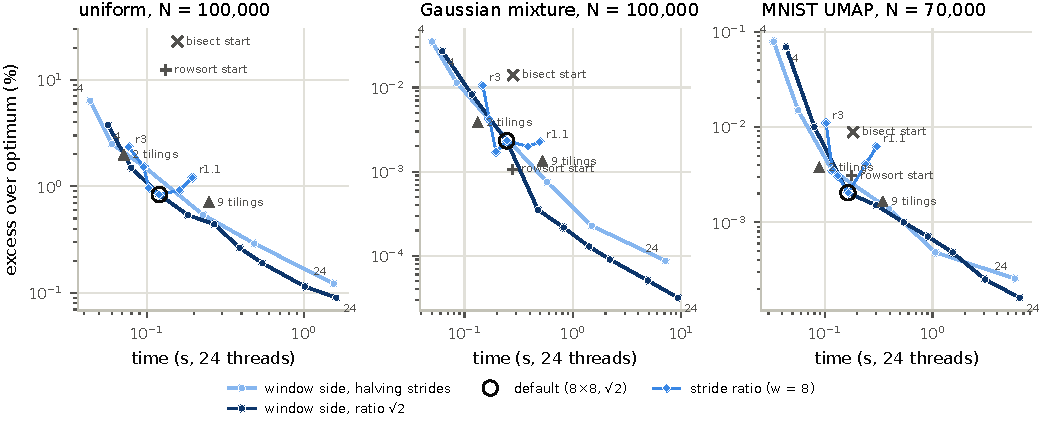
\includegraphics[width=\linewidth]{figures/fig_ablation.pdf}
  \caption{Held-out ablations. Each panel shows mean excess over the certified optimum against
  median time (24 threads, three instance seeds). Lines vary an ordered setting of the
  baseline: the window side, with halving (light) or $\sqrt2$ strides (dark), labelled
  by the side length; and the stride ratio at $w=6$ (diamonds; r3 and r1.1 mark the
  extremes). Markers show categorical changes to the baseline: bisection or row-sort
  starts, and 2 or 9 shifted tilings per round instead of 4. A single tiling
  ($>$20{,}000\% on uniform points) is off the chart. Solver choice and skipping unchanged
  windows do not change quality; they are listed with all other numbers in
  Table~\ref{tab:ablation}.}
  \label{fig:ablation}
\end{figure}

Figure~\ref{fig:ablation} varies one design choice at a time, starting from the baseline,
on instances that were not used for any design decision.
\begin{itemize}
\item \textbf{Window side} is the main quality knob. With halving strides, uniform
  excess falls from 15.7\% ($3\times3$) to 2.5\% ($6\times6$), 0.54\% ($12\times12$) and
  0.29\% ($16\times16$). Time rises from 0.05\,s to 1.5\,s on uniform points and from
  0.07\,s to 8.4\,s on the mixture. The $\sqrt2$ schedule shifts the whole curve down
  (e.g.\ 1.5\% at $6\times6$).
\item \textbf{Stride ratio}. $\sqrt2$ is best or close to best on all three inputs: on
  uniform points 1.5\% against 2.5\% for halving and 4.1\% for a ratio of 3, and 1.9\%
  for the finest ratio tested, 1.1. Finer is not always better.
\item \textbf{Coarse levels are essential}. Capping the first stride at 16, 8, 4, 2 or 1 (the
  last means stride-1 windows only, from the random start) made results 5--37$\times$
  worse and 5--90$\times$ slower. With halving from the automatic first stride of 64,
  uniform excess is 2.5\% in 0.12\,s; capped at 16 it is 11.7\% in 0.57\,s, and with
  stride 1 only it is 27\% in 1.3\,s. Without long-range moves, stride-1 windows need many
  rounds to repair a random start, and they stall far from the optimum.
\item \textbf{Start}. A random start beats bisection and row sorting by 4--18$\times$ (uniform:
  2.5\% against 29.9\% and 22.9\%). Better-looking starts contain straight seams that
  windows cannot undo.
\item \textbf{Shifted tilings are essential}. With a single fixed tiling, points can never
  cross a window border, and the method fails (uniform: excess over 20{,}000\%). Two
  diagonal shifts give 5.5\%, the four of the baseline 2.5\%, and nine shifts 1.9\% at
  twice the time. More rounds per level help about as much per second as larger windows
  (two rounds: 2.1\% at 1.4$\times$ the time).
\item \textbf{Window solver}. All three solvers are exact, so the assignments are
  identical. Jonker--Volgenant is 2--10$\times$ slower than the Hungarian method. The
  greedy warm start saves up to 15\% on uniform inputs but is 2--3\% slower on the
  clustered ones, so its benefit in the micro-benchmark (5--20\%) does not carry over
  consistently.
\item \textbf{Skipping unchanged windows} leaves results unchanged and saves 35--40\% of the time.
\item \textbf{Post-processing does not pay.} Three extra cycles of stride-2 and stride-1
  rounds after convergence changed nothing on uniform points and removed under 3\% of the
  excess on the clustered inputs. Merging four independent baseline runs, keeping the
  cheaper of the two assignments on every connected component of their union (the rule
  BSP-OT uses to merge plans), cut the uniform excess by 23--38\% at four times the cost.
  The fast preset does better (1.5\%) at about the same cost as the baseline on these
  uniform instances.
\end{itemize}
